
\section{Sistema di autenticazione}

Il sistema di autenticazione si occupa di gestire gli account degli utenti, di autenticarli e di autorizzarli a compiere determinate azioni.

\paragraph{Obiettivo} Il sistema di autenticazione si propone come goal principale quello di offrire all'utente non autenticato la possibilità di autenticarsi, questa condizione viene poi utilizzata come precondizione in molti degli altri sistemi e casi d'uso.

\begin{figure}[h]
    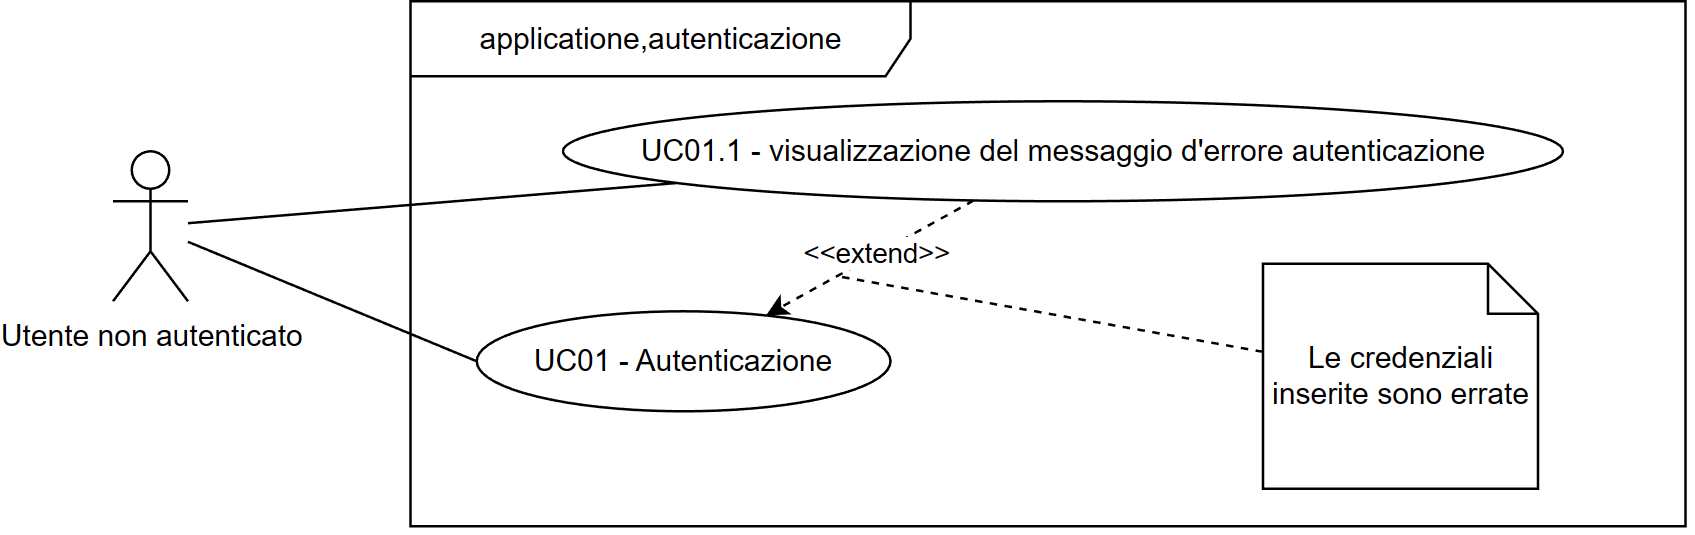
\includegraphics[width=\textwidth]{contenuti/img/casi_uso_grafici-applicazione,autenticazione.png}
    \caption{Parte relativa all'autenticazione dell'applicazione}
    \label{fig:autenticazione}
\end{figure}

\subsection{I casi d'uso descritti}

\begin{itemize}
    \item UC01
    \item UC01.1
\end{itemize}